\documentclass{article} %[letterpaper,11pt]
\usepackage{graphicx}
\usepackage{caption}
\usepackage{subcaption}
\usepackage{url}

\usepackage{amsmath}

\newcommand{\code}[1]{\texttt{#1}}
\renewcommand\refname{5  \hspace{4 mm}References}

\begin{document}

\title{CS 867: Program 3}
\date{October 20, 2013}
\author{Carmen St.\ Jean}

\maketitle

\section{Introduction}

Since its introduction in 1786 by Playfair \cite{playfair1786}, the line chart has been the conventional choice for visualization of temporal data in different fields such as medicine, economics, and ecology.  Though line charts are quite popular, perhaps alternatives might be better suited for depicting time-oriented data in an understandable manner, especially if a specific set of perceptual tasks are expected be performed on the data.  This paper is a review of two approaches to alternative visualizations to the traditional line chart.

\section{Background}

\begin{figure}
        \centering
        \begin{subfigure}[b]{0.45\textwidth}
                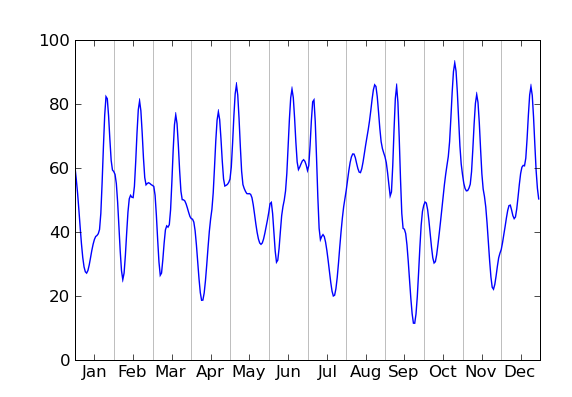
\includegraphics[width=\textwidth]{figures/conditions-a.png}
                \caption{An ordered line chart.}
                \label{fig:avg_line}
        \end{subfigure}
        \begin{subfigure}[b]{0.45\textwidth}
                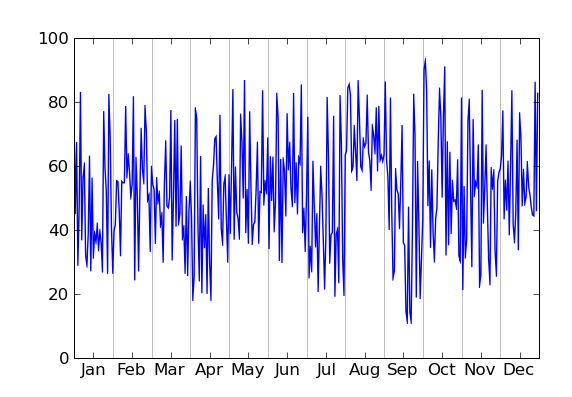
\includegraphics[width=\textwidth]{figures/conditions-b.png}
                \caption{A 1D permuted line chart}
                \label{fig:avg_line_p}
        \end{subfigure}
        \\
        \begin{subfigure}[b]{0.45\textwidth}
                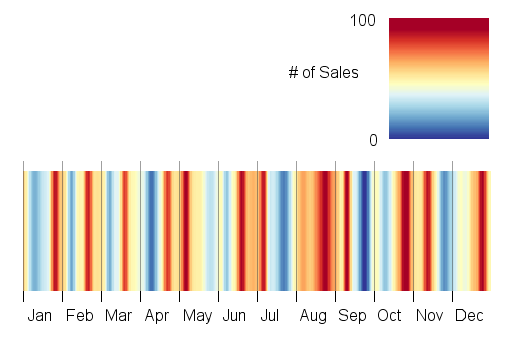
\includegraphics[width=\textwidth]{figures/conditions-c.png}
                \caption{An ordered colorfield.}
                \label{fig:avg_color}
        \end{subfigure}
        \begin{subfigure}[b]{0.45\textwidth}
                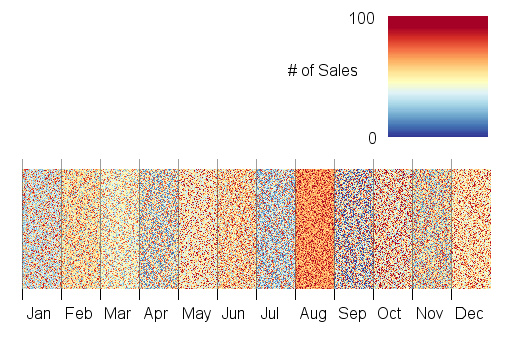
\includegraphics[width=\textwidth]{figures/conditions-d.png}
                \caption{A 2D permuted colorfield.}
                \label{fig:avg_color_p}
        \end{subfigure}
        \caption{Four possible visualizations for aggregate tasks \cite{correll2012}.}
        \label{fig:avg}
\end{figure}

Shneiderman's ``overview first, details on demand'' mantra \cite{shneiderman1996} was the basis of the approach taken by Correll et al.: design a visualization of aggregate data that will make use of pre-attentive processing \cite{correll2012}.  Their reasoning was that sub-ranges often need identification---e.g., which month had the highest average of sales for the company?   Therefore, Correll et al. proposed the use of colorfields, which use color rather than $y$-position to encode a variable, as seen in Figure~\ref{fig:avg_color}.  This was evaluated against the line chart and ``permuted'' versions of the colorfield---where the $x$- and $y$-positions of the pixels were randomly permuted within each month, seen in Figure~\ref{fig:avg_color_p}---and of the line chart---where the $x$-positions were randomly permuted within each month, seen in Figure~\ref{fig:avg_line_p}.

\begin{figure}
        \centering
        \begin{subfigure}[b]{0.4\textwidth}
                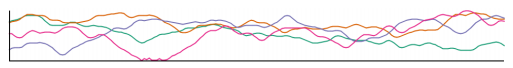
\includegraphics[width=\textwidth]{figures/ts_simplelinegraph.png}
                \caption{A simple line graph.}
                \label{fig:ts_simple}
        \end{subfigure}
        \begin{subfigure}[b]{0.4\textwidth}
                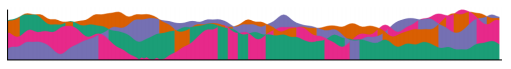
\includegraphics[width=\textwidth]{figures/ts_braidedgraph.png}
                \caption{A braided graph.}
                \label{fig:ts_braid}
        \end{subfigure}
        \\
        \begin{subfigure}[b]{0.4\textwidth}
                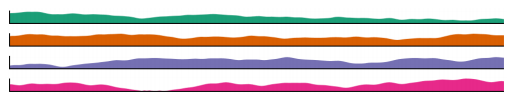
\includegraphics[width=\textwidth]{figures/ts_smallmultiples.png}
                \caption{Small multiples.}
                \label{fig:ts_smmult}
        \end{subfigure}
        \begin{subfigure}[b]{0.4\textwidth}
                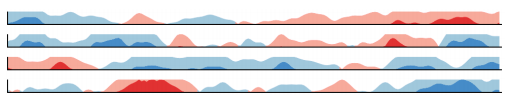
\includegraphics[width=\textwidth]{figures/ts_horizongraphs.png}
                \caption{Horizon graphs.}
                \label{fig:ts_horizon}
        \end{subfigure}
        \caption{Four possible methods for visualizing multiple time series \cite{javed2010}.}
        \label{fig:ts_compare}
\end{figure}

On the other hand, Javed et al. designed their alternatives with the idea that several concurrent time series often need to be viewed and compared.

\bibliographystyle{plain}

\bibliography{sources}

\end{document}

